\section{Introduction}
The Cabibbo-favored (CF) $D_{s}^{+} \rightarrow K^{+}K^{-}\pi^{+}$ decay has a large branching fraction and low background contamination.
This decay is, therefore, usually suited as a reference channel for other decays of the $D_{s}$ meson and used as normalization for decay chains involving charm quarks.
An accurate knowledge of its substructure is important to reduce systematic uncertainties in analyses using this channel.
The study of intermediate processes in this decay can also illuminates light meson spectroscopy and shed light on different production mechanisms.
\subsection{The Scalar Mesons $f_{0}(980)$ and $a_{0}(980)$}
\label{f0-a0-discussion}
\par{
    The Constituent Quark Model has been very successful in the past few decades by explaining how hadrons are made up.
    Based on this model, the nonets of pseudo-scalar, vector, and tensor mesons are now well identified.
    However, the identification of the scalar mesons is still uncertain due to the broad widths and the lack of a distinctive angular distribution.
    Among the candidates for the spin-parity $J^{PC}=0^{++}$ nonet, the parameters of some states such as $f_{0}(980)$ and $a_{0}(980)$ are not well measured,
    
    %its parameters are still uncertain.
    
    
    Recently, the decay $D_{s}^{+} \rightarrow a_{0}(980)^{0}\pi^{+}$ has been observed through $D_{s}^{+} \rightarrow \pi^{+}\pi^{0}\eta$~\cite{Doc-DB-682-v7}.
    %According to the amplitude analysis of $D_{s}^{+} \rightarrow \pi^{+}\pi^{0}\eta$~\cite{Doc-DB-682-v7}, the decay $D_{s}^{+} \rightarrow a_{0}(980)^{0}\pi^{+}$ is observed.
    The overlap of $f_{0}(980)$ and $a_{0}(980)$ makes it very difficult to distinguish them (Appendix ~\ref{app:a0_f0_dis}).
    %However, $f_{0}(980)$ and $a_{0}(980)$ are very close to each other and it is very difficult to distinguish them.
    From the Dalitz plot analysis of $D_{s}^{+} \rightarrow \pi^{+}\pi^{-}\pi^{+}$, we can get the branching fraction $\mathcal{B}(D_{s}^{+} \rightarrow f_{0}(980)\pi^{+}, f_{0}(980) \rightarrow \pi^{+}\pi^{-})$.
    With the branching ratio of $\Gamma_{f_{0}(980)}(K^{+}K^{-})/\Gamma_{f_{0}(980)}(\pi^{+}\pi^{-})$, we can obtain:
    \begin{equation}
        %\begin{math}
            \mathcal{B}(D_{s}^{+} \rightarrow f_{0}(980)\pi^{+}, f_{0}(980) \rightarrow K^{+}K^{-}) =\mathcal{B}(D_{s}^{+} \rightarrow f_{0}(980)\pi^{+}, f_{0}(980) \rightarrow \pi^{+}\pi^{-})  \frac{\Gamma_{f_{0}(980)}(K^{+}K^{-})}{ \Gamma_{f_{0}(980)}(\pi^{+}\pi^{-})}. \label{bf-f0}
        %\end{math}
    \end{equation}
    
    In a similar way, we can obtain:
    \begin{equation}
        %\begin{math}
            \mathcal{B}(D_{s}^{+} \rightarrow a_{0}(980)\pi^{+}, a_{0}(980) \rightarrow K^{+}K^{-}) =\mathcal{B}(D_{s}^{+} \rightarrow a_{0}(980)\pi^{+}, a_{0}(980) \rightarrow \pi^{0}\eta)  \frac{\Gamma_{a_{0}(980)}(K^{+}K^{-})}{ \Gamma_{a_{0}(980)}(\pi^{0}\eta)}. \label{bf-a0} 
        %\end{math}
    \end{equation}
    
    So the ratio of fit fractions, $\mathcal{R}$, between $D_{s}^{+} \rightarrow f_{0}(980)\pi^{+}$ and $D_{s}^{+} \rightarrow a_{0}(980)\pi^{+}$ in the final state is: 
    \begin{equation}
        %\begin{math}
        \mathcal{R}  =\frac{\mathcal{B}(D_{s}^{+} \rightarrow f_{0}(980)\pi^{+}, f_{0}(980) \rightarrow \pi^{+}\pi^{-})  \frac{\Gamma_{f_{0}(980)}(K^{+}K^{-})}{ \Gamma_{f_{0}(980)}(\pi^{+}\pi^{-})}}{\mathcal{B}(D_{s}^{+} \rightarrow a_{0}(980)\pi^{+}, a_{0}(980) \rightarrow \pi^{0}\eta)  \frac{\Gamma_{a_{0}(980)}(K^{+}K^{-})}{ \Gamma_{a_{0}(980)}(\pi^{0}\eta)}}. \label{a0-f0-bf}
        %\end{math}
    \end{equation}
    
    The confirmation of the value $\mathcal{R}$ in Eq.~\ref{a0-f0-bf} can help to fix the ratio in amplitude analyses and then distinguish $f_{0}(980)$ and $a_{0}(980)$ at the low end of $K^{+}K^{-}$ mass spectrum.
    Using isospin relations,  the relation between $\Gamma_{f_{0}(980)}(\pi\pi) /  \Gamma_{f_{0}(980)}(\pi\pi+K\bar{K})$ and $\Gamma_{f_{0}(980)}(K^{+}K^{-}) / \Gamma_{f_{0}(980)}(\pi^{+}\pi^{-})$ is:
    \begin{equation}
        \frac{\Gamma_{f_{0}(980)}(K^{+}K^{-})}{ \Gamma_{f_{0}(980)}(\pi^{+}\pi^{-})} =  \frac{3}{4} \cdot \left[\frac{1}{\frac{\Gamma_{f_{0}(980)}(\pi\pi)} {\Gamma_{f_{0}(980)}(\pi\pi)+\Gamma_{f_{0}(980)}(K\bar{K})}} -1\right]. \label{f0-KK-pipi-relation}
    \end{equation}
    However, the value of $\Gamma_{f_{0}(980)}(K^{+}K^{-}) / \Gamma_{f_{0}(980)}(\pi^{+}\pi^{-})$ is not well measured, shown in Table~\ref{f0-KK-pipi}. %~\cite{PDG2018}.
    $f_{0}(980)$ is very close to $K\bar{K}$ threshold and has strong coupling to $\pi\pi$ and $K\bar{K}$ final states.
    So, in this analysis, we use $S(980)$ to denote the $a_{0}(980)$ and $f_{0}(980)$ resonances in Sec.~\ref{Amplitude-Analysis}.
    And we perform a model-independent partial wave analysis (MIPWA) to extract the $S(980)$ lineshape in the low end of $K^{+}K^{-}$ mass spectrum (Sec.~\ref{MIPWA}). %in a quasi-model-independent way.
    
    %In other words, we take $a_{0}(980)$ and $f_{0}(980)$ as a whole in amplitude analysis.

\begin{table}[htbp]
    \caption{The $f_{0}(980)$ branching ratio $\Gamma_{f_{0}(980)}(\pi\pi) / \left[ \Gamma_{f_{0}(980)}(\pi\pi)+\Gamma_{f_{0}(980)}(K\bar{K})\right]$}
    \label{f0-KK-pipi}
    \begin{center}
        \begin{tabular}{cccc}
            \toprule
            value &         Collaboration & comment\\
            \hline
            $0.52\pm0.12$ &             BABAR    & $B^{\pm} \rightarrow K^{\pm}\pi^{\pm}\pi^{\mp}$  ~\cite{pipi-KK-1} \\
            $0.75_{-0.13}^{+0.11}$ &    BESII    & $\chi_{c0} \rightarrow 2\pi^{+}2\pi^{-}, \pi^{+}\pi^{-}K^{+}K^{-}$  ~\cite{pipi-KK-2} \\
            $0.84\pm0.02$ &             SPEC    & Combined fit  ~\cite{pipi-KK-3} \\
            \bottomrule
        \end{tabular}
    \end{center}
\end{table}





}

\subsection{The Dynamics of the Strong Interaction}
%\subsection{The $D_{s}^{+} \rightarrow K^{+}K^{-}\pi^{+}$ decay}
\par{
    Hadronic decays of charmed mesons are important for understanding the dynamics of the strong interaction in the low energy regime.
    Fig.~\ref{Feynman-dia} illustrates main Feynman diagrams related to the $D_{s}^{+} \rightarrow K^{+}K^{-}\pi^{+}$ decay.
    Experimental measurements can help to refine theoretical models~\cite{PRD93-114010}.
    Table~\ref{theory-pre} shows the predictions of the branching fractions of $D_{s}^{+} \rightarrow \bar{K}^{*}(892)^{0}K^{+}$ and $D_{s}^{+} \rightarrow \phi(1020)\pi^{+}$.
    \begin{table}[htbp]
        \caption{
            $\mathcal{B}(A1)$, $\mathcal{B}(S4)$, $\mathcal{B}(pole)$ and $\mathcal{B}(FAT[mix])$ are 4 theory predictions~\cite{PRD93-114010}. 
        }
        \label{theory-pre}
        \begin{center}
            \begin{tabular}{cccccccc}
                \toprule\toprule
                Mode &  $\mathcal{B}(A1)$ (\%)& $\mathcal{B}(S4)$ (\%)&  $\mathcal{B}(pole)$ (\%)&$\mathcal{B}(FAT[mix])$ (\%)&\\
                $D_{s}^{+} \rightarrow \bar{K}^{*}(892)^{0}K^{+}$           & $3.92\ \pm\ 1.13$  & $3.93\ \pm\ 1.10$  & $4.2\ \pm\ 1.7$  & $4.07$  \\
                $D_{s}^{+} \rightarrow \phi(1020)\pi^{+}$                   & $4.49\ \pm\ 0.40$  & $4.51\ \pm\ 0.43$  & $4.3\ \pm\ 0.6$  & $3.4$  \\
                %Mode & $\mathcal{B}(exp)$ (\%)   & $\mathcal{B}(A1)$ (\%)& $\mathcal{B}(S4)$ (\%)& $\mathcal{B}(pole)$ (\%)& $\mathcal{B}(FAT[mix])$ (\%) \\
                %$D_{s}^{+} \rightarrow \bar{K}^{*}(892)^{0}K^{+}$           & $3.94\ \pm\ 0.12$    & $3.92\ \pm\ 1.13$  & $3.93\ \pm\ 1.10$  & $4.2\ \pm\ 1.7$  & $4.07$\\
                %$D_{s}^{+} \rightarrow \phi(1020)\pi^{+}$                   & $4.60\ \pm\ 0.17$    & $4.49\ \pm\ 0.40$  & $4.51\ \pm\ 0.43$  & $4.3\ \pm\ 0.6$  & $3.4$\\
                \hline
                \bottomrule\bottomrule
            \end{tabular}
        \end{center}
    \end{table}
    \begin{figure*}[htbp]
        \centering
        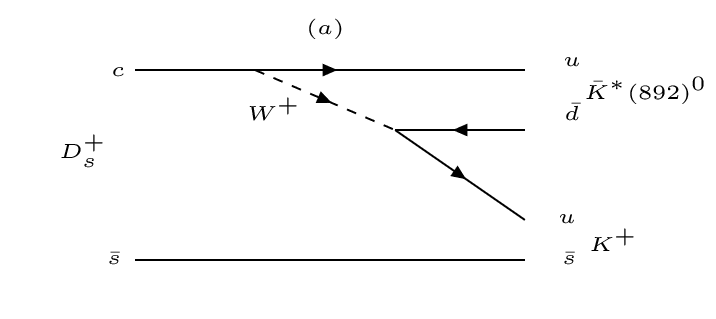
\includegraphics[width=0.45\textwidth]{plot/Fa.PNG}
        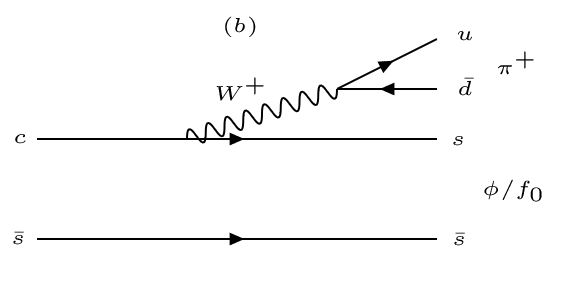
\includegraphics[width=0.45\textwidth]{plot/Fb.PNG}
        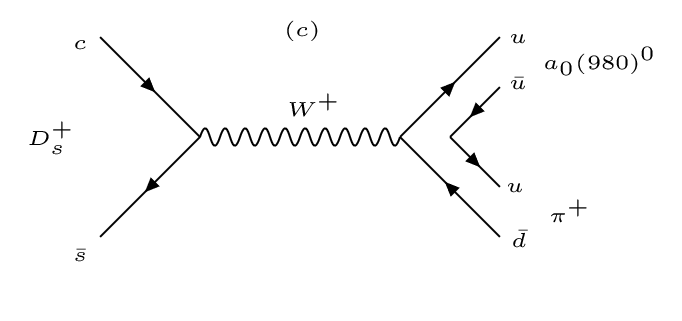
\includegraphics[width=0.45\textwidth]{plot/Fc.PNG}
        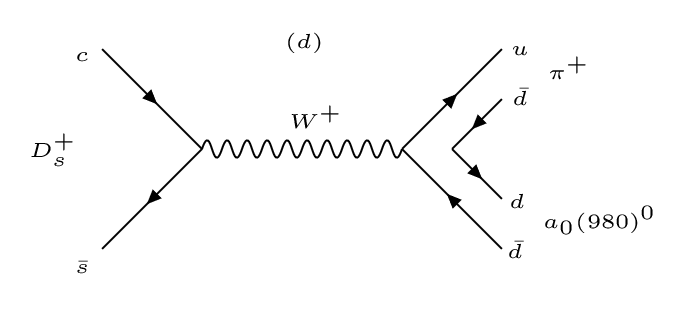
\includegraphics[width=0.45\textwidth]{plot/Fd.PNG}
        %\includeraphics[width=0.45\textwidth]{plot/Fe.PNG}
        \caption{
        Main decay diagrams associated with $D_{s}^{+} \rightarrow K^{+}K^{-}\pi^{+}$ decay.
    The main contribution comes from the tree diagram with an internal $W^{+}$ emission (Fig.~\ref{Feynman-dia}(a)), that describes the $D_{s}^{+} \rightarrow \bar{K}^{*}(892)^{0}K^{+}$ decay, 
    the diagram with an external $W^{+}$ emission (Fig.~\ref{Feynman-dia}(b)), that describes the diagram $D_{s}^{+} \rightarrow \phi\pi^{+}/ f_{0}\pi^{+}$, 
    and the diagram with W-annihilation (Fig.~\ref{Feynman-dia}(c) and Fig.~\ref{Feynman-dia}(d)), that describes the decay $D_{s} \rightarrow a_{0}(980)^{0}\pi^{+}$.
    }
        \label{Feynman-dia}
    \end{figure*}
    
    
}
    
\subsection{Amplitude Analysis}
\par{
    Knowledge of the substructures in $D_{s}^{+} \rightarrow K^{+}K^{-}\pi^{+}$ decay allows us to properly determine the detection efficiency when measuring its branching fraction.
    Dalitz plot analyses of this decay have been performed by the E687~\cite{E687RES}, CLEO ~\cite{2009CLEO} and Babar~\cite{2011BARBAR} collaborations.
    E687 used about 700 events and did not take $f_{0}(1370)\pi^{+}$ into account. 
    For CLEO-c, about 14400 events with purity about 84.9\% were selected with the single tag method.
    The analysis of BARBAR used about 100000 events with purity about 95\%. 
    Table~\ref{PreviousAnalyses} shows the comparision of the fitted decay fractions with the Dalitz plot analyses of previous analyses.
}

\begin{table}[htbp]
    \caption{Comparison between Babar, CLEO-c and E687 Dalitz plot analysis.}
    \label{PreviousAnalyses}
    \begin{center}
        \begin{tabular}{cccc}
            \toprule\toprule
            Decay mode & Fit fraction(BABAR)  & Fit fraction(CLEO-c)  & Fit fraction(E687)\\
            \midrule
            $D_{s}^{+} \rightarrow \bar{K}^{*}(892)^{0}K^{+}$              & 47.9$\pm$0.5$\pm$0.5  & 47.4$\pm$1.5$\pm$0.4& 47.8$\pm$4.6$\pm$4.0 \\
            $D_{s}^{+} \rightarrow \phi(1020)\pi^{+}$                      & 41.4$\pm$0.8$\pm$0.5  & 42.2$\pm$1.6$\pm$0.3& 39.6$\pm$3.3$\pm$4.7 \\
            $D_{s}^{+} \rightarrow S(980)\pi^{+}$    & 16.4$\pm$0.7$\pm$2.0  & 28.2$\pm$1.9$\pm$1.8& 11.0$\pm$3.5$\pm$2.6 \\
            %$D_{s}^{+} \rightarrow f_{0}(980)\pi^{+}/a_{0}(980)\pi^{+}$    & 16.4$\pm$0.7$\pm$2.0  & 28.2$\pm$1.9$\pm$1.8& 11.0$\pm$3.5$\pm$2.6 \\
            $D_{s}^{+} \rightarrow \bar{K}^{*}_{0}(1430)^{0}K^{+}$         & 2.4$\pm$0.3$\pm$1.0   & 3.9$\pm$0.5$\pm$0.5 & 9.3$\pm$3.2$\pm$3.2  \\
            $D_{s}^{+} \rightarrow f_{0}(1710)\pi^{+}$                     & 1.1$\pm$0.1$\pm$0.1   & 3.4$\pm$0.5$\pm$0.3 & 3.4$\pm$2.3$\pm$3.5  \\
            $D_{s}^{+} \rightarrow f_{0}(1370)\pi^{+}$                     & 1.1$\pm$0.1$\pm$0.2   & 4.3$\pm$0.6$\pm$0.5 & ...                  \\ 
            $\begin{matrix}\sum FF(\%)\end{matrix}$                          & 110.2$\pm$0.6$\pm$2.0 & 129.5$\pm$4.4$\pm$2.0 & 111.1\\
                \midrule
                $\chi^{2}/NDF$                                                  & $\frac{2843}{2305-14}=1.2$ & $\frac{178}{117}=1.5$ & $\frac{50.2}{33}=1.5$\\
                \midrule
                Events                                                         &$96307\pm369$          &$12226\pm22$  &$701\pm36$\\
                \bottomrule\bottomrule
            \end{tabular}
        \end{center}
    \end{table}
    From Table~\ref{PreviousAnalyses}, we can see an obvious difference of decay fraction of $S(980)\pi^{+}$ between BABAR and CLEO-c.  
    In this analysis with the double tag method, we can get a nearly background free data sample, which is good to perform the amplitude analysis.

    \iffalse
    As shown in Fig.~\ref{fig:lambc_cs} and Figure~\ref{fig:lambc_cs_bes3}, at the energy of 4.6\,GeV, cross section of producing $\lambdacp\lambdacm$ pair in $\ee$ collisions is $\sigma(\ee\to\lambdacp\lambdacm)=0.38\pm0.13\,\rm{nb}$ measured by BELLE~\cite{Pakhlova:2008vn} and $\sigma(\ee\to\lambdacp\lambdacm)=0.253\pm0.023\,\rm{nb}$ measured by BESIII~\cite{Weiping:lineshape}.\\

    %%%%%%%%%%%%%%%%%%%%%%%%%%%%


    %%%%%%%%%%%%%%%%%%%%%%%%%%%%
    \begin{figure*}[htbp]
        \centering
        \includegraphics[width=0.45\textwidth]{bes3_lineshape.eps}
        \caption{Cross sections of $\ee\to\lambdacp\lambdacm$ measured by BESIII.}
        \label{fig:lambc_cs_bes3}
    \end{figure*}
    %%%%%%%%%%%%%%%%%%%%%%%%%%%%%
    \fi
